\documentclass[authoryear]{elsarticle}



%Automatically load natbib


\usepackage{lineno}

\modulolinenumbers[5]

%\usepackage[utf8]{inputenc} 
%\usepackage[T1]{fontenc}
%\usepackage[top=2cm, bottom=2cm, left=2.5cm, right=2.5cm]{geometry}
\usepackage{amsmath,amsfonts,amssymb}
\usepackage{graphicx}
\usepackage{eurosym}

\usepackage[titletoc,title]{appendix}
\usepackage{booktabs}
\usepackage{caption}
\usepackage{subcaption}
\usepackage{multirow}
\usepackage[table]{xcolor}
\usepackage{pdflscape}
\usepackage{rotating}
\usepackage{tabularx}
\usepackage{tabulary}
\usepackage{afterpage}
\usepackage{ulem}

\usepackage{colortbl}
\newcommand\colorTable{\rowcolors{1}{white}{blue!20}}
\textwidth=15cm
\usepackage[textsize=small,textwidth=2.9cm,shadow]{todonotes}

\usepackage{hyperref}

\usepackage{cleveref}




%\bibliographystyle{plainnat}
\bibliographystyle{elsarticle-harv}
%\bibliographystyle{elsarticle-harv-no_url}
%\bibliographystyle{elsarticle-num-names-no_url}


%\journal{Journal of \LaTeX\ Templates}

%%%%%%%%%%%%%%%%%%%%%%%
%% Elsevier bibliography styles
%%%%%%%%%%%%%%%%%%%%%%%
%% To change the style, put a % in front of the second line of the current style and
%% remove the % from the second line of the style you would like to use.
%%%%%%%%%%%%%%%%%%%%%%%

%% Numbered
%\bibliographystyle{model1-num-names}

%% Numbered without titles
%\bibliographystyle{model1a-num-names}

%% Harvard
%\bibliographystyle{model2-names.bst}\biboptions{authoryear}

%% Vancouver numbered
%\usepackage{numcompress}\bibliographystyle{model3-num-names}

%% Vancouver name/year
%\usepackage{numcompress}\bibliographystyle{model4-names}\biboptions{authoryear}

%% APA style
%\bibliographystyle{model5-names}\biboptions{authoryear}

%% AMA style
%\usepackage{numcompress}\bibliographystyle{model6-num-names}

%% `Elsevier LaTeX' style
%\bibliographystyle{elsarticle-num}

%%%%%%%%%%%%%%%%%%%%%%%

\newcommand\eff{\textsc{Eff}}
\newcommand\emwh{\euro/MWh}
\newcommand\lcoe{\textsc{lcoe}}
\newcommand\dnte{\textsc{dnte}}
\newcommand\lcoen{\lcoe$_\text{N}$}
\newcommand\lcoer{\lcoe$_\text{R}$}
\newcommand\coo{CO\textsubscript{2}}

%Pour enlever la note de bas de page "Preprint submitted to Elsevier, cf https://tex.stackexchange.com/questions/35712/modify-footer-used-by-elsarticle-cls
\usepackage{etoolbox}
\makeatletter
\patchcmd{\ps@pprintTitle}{\footnotesize\itshape
	Preprint submitted to \ifx\@journal\@empty Elsevier
	\else\@journal\fi\hfill\today}{\relax}{}{}
\makeatother

%\usepackage{Sweave}
\begin{document}
%\input{documentation-concordance}
	
	
\title{The FLORE model: Model documentation}


\author[mymainaddress]{Quentin Perrier\corref{mycorrespondingauthor}}
\cortext[mycorrespondingauthor]{Corresponding author. E-mail address: \url{perrier@centre-cired.fr}}


\address[mymainaddress]{CIRED, 45 bis, avenue de la Belle Gabrielle, 94736 Nogent-sur-Marne Cedex, France}

\begin{frontmatter}
	
	\begin{abstract}
This paper documents the FLORE model, a model of power system optimization for France using GAMS.		
	\end{abstract}
	
	\begin{keyword}
		Power system \sep Nuclear power \sep Uncertainty \sep Investment optimization \sep Robust Decision Making 
		%\MSC[2010] 00-01\sep  99-00
	\end{keyword}
	
\end{frontmatter}

\tableofcontents

\clearpage

\section{Overview}
The French power model FLORE is a dispatch and investment model of the French power mix. It is a partial equilibrium model of the wholesale electricity market, which determines optimal investment and hourly generation.

FLORE minimizes total cost with respect to investment and production under a set of constraints. The model is linear, deterministic, and solved in hourly time step for each year, from 2014 to 2050.

Generation is modelled as twelve distinct technologies: three Variable Renewable Electricity sources (VRE) with zero marginal costs - onshore wind, offshore wind and solar, three fossil-based thermal technologies - coal, combined cycle gas turbine (CCGT), open cycle gas turbine (OCGT), three nuclear technologies (historical nuclear, retrofitted nuclear and new nuclear), and three hydro systems - run-of-river, conventional dams (lakes) and pumped storage. 
Hourly VRE generation is limited by specific generation profiles.
Dispatchable power plants produce whenever the price is above their variable costs, and unless they are limited by their ramping constraints.
Hydro storage and dispatch is optimized by the model, under water reservoir constraints and pumping losses.
At the end its lifetime, each capacity is decommissioned.

A particularity of the model is to represent explicitly the cost of extending the lifetime of nuclear power plants. Nuclear plants normally close after 40 years, but their lifetime can be extended to 60 years, if upgrade costs are paid for.

Demand is exogenous and assumed to be perfectly price inelastic at all times.

FLORE is currently calibrated for France. Exports are given exogenously.

\section{Total System Costs}

The model minimizes total system costs $C$ with respect to several constraints and decision variables. Total system costs are the sum of fixed costs (representing the sum of capital and fixed O\&M costs), and variable costs, over all hours $h$, weeks $w$, years $y$ and generation technologies $tec$. 

Throughout this model description, names in full capital letters denote a choice variable for the model, while names with lowercase letters denote an exogenous data or parameter.

Fixed costs per unit of capacity installed, for each technology in year $y$, is equal to its annualized capacity cost $capex(tec)$ plus fixed O\&M costs $fixedOM(tec)$. 
\begin{equation*}
fixedCosts(tec) = capex(tec) + 	fixedOM(tec) \quad \text{(in keuros/GW)}
\end{equation*}
Variable generation costs per unit of production are equal to the fuel costs, in euros/MWh, divided by the efficiency of the plant, plus the CO\textsubscript{2} content of the fuel, multiplied by the CO\textsubscript{2} price of the plant, and divided by its efficiency.
\begin{equation*}
variableCosts_{year,tec} = \frac{ fuelCosts_{year,tec} + CO2content_{tec} \cdot CO2price_{year} } {Efficiency_{year, tec}} \quad \text{(in keuro/GWh)}
\end{equation*}
To account for the fact that we have only 12 representative weeks, we multiple the variable costs by $\frac{365}{6*7}$ (the denominator indicates 6 representative weeks of 7 days) to get total annual variable costs. Total cost is thus equal to:
\begin{equation}
COST =\sum_{tec,y} CAPA_{tec,y} \cdot fixedCosts_{tec} + \sum_{tec,y,w,h} GENE_{tec,y,w,h} \cdot variableCosts_{year,tec} * \frac{365}{42}
\end{equation}
This total cost is the objective function to be minimized.

\section{Supply and demand}

Power balance between supply and demand is the central constraint of the model. 
Total demand is the sum of national consumption $consumption(y,w,h)$, pumping for pumped-storage hydro $PUMP(y,w,h)$ and net export flows $exports(y,w,h)$. 
Supply is the sum of generation over all technologies.
The balance between supply and demand is thus equal to:
\begin{equation}
  \forall(y,w,h) \quad \sum_{tec} GENE(tec,y,w,h) \geq \sum_{tec} consumption(y,w,h)   + exports(y,w,h) + PUMP(h,y)
\end{equation}

In this framework, demand is perfectly price-inelastic. Cost minimization is thus equivalent to welfare-maximization.

Generation of dispatchable capacities is constrained by capacities installed and the load factor (also called availability), minus the capacity which is booked for reserve requirements. 
For non-dispatchable technologies (wind, PV and run-of-river hydro), generation is limited by an hourly generation profile.
\begin{multline}
  GENE(tec\_dispa,y,w,h)      \leq  CAPA(tec\_dispa,y)*loadfactor(w,tec\_dispa) \\ - RES(tec\_dispa,y,w,h)
\end{multline}
For wind and PV, a generation profile is an additional constraint:
\begin{equation}
  GENE(tec\_vre,y,w,h)        \leq  CAPA(tec\_vre,y)*vre\_profiles(tec\_vre,w,h) 
\end{equation}
For run-of-river hydro, generation is fixed exogenously for each week:
\begin{equation}
  \sum_h GENE('lake',y,w,h) \leq lake_inflows(w) ;
\end{equation}

\section{Investment}

Regarding capacities, investment is exogenous for historical nuclear and the three hydro technologies: run-of-river, lake dams and pumped hydro.
The capacity of historical nuclear technology is decreasing based on plant-level data. 

The capacity of all other technologies is determined endogenously by the model. Capacity is installed when optimal, and then decommissioned when it reaches its lifetime. The initial capacity is supposed to be decommissioned linearly from the initial capacity in a period of 40 years.
\begin{equation}
CAPA(tec\_end,y+1) = CAPA(tec\_end,y) + INVE(tec\_end,y) - DECO(tec\_end,y)
\end{equation}

\begin{multline}
DECO(tec\_end,y) = INVE(tec\_end,y-lifetime(tec\_end))\$(ord(y)>lifetime(tec\_end)) \\ + (init\_cap(tec\_end)/40)\$(ord(y) \leq 40)
\end{multline}

The amount of investment in retrofitting capacities cannot exceed the existing historical capacity. When historical capacity reaches the end of its initial lifetime, it can be either decomissionned or retrofitted:
\begin{equation}
INVE('nuc\_retrofit',y) \leq CAPA('nuc\_hist',y) - CAPA('nuc\_hist',y+1)
\end{equation}

Finally, we set on a cap on the maximum capacity than can be installed each year:
\begin{align}
& INVE('onshore',y) \leq  4 \\
& INVE('nuc\_new',y) \leq  5
\end{align}


\section{Hydropower}

The pumping is bounded by the available pumping capacity:
\begin{equation}
pump\_cap(y) \geq  PUMP(y,w,h)
\end{equation}
The pumping generates energy losses of about 20\%:
\begin{equation}
0.8*\sum_h PUMP(y,w,h) \geq \sum_h GENE('step',y,w,h)
\end{equation}

Finally, the amount of pumped water and hydro generation is constrained by the water reservoir capacities. We assume that the reservoir start each month by being three quarters full.
The reservoir capacities are approximately equal to twenty hours of pumping.

Pumping is limited by the reservoir capacities (no spill allowed):

\begin{equation}
20*pump\_cap(y)*(1/4) \geq \sum_{i\$(ord(i)<ord(h))} 0.8*PUMP(y,w,i)-GENE('step',y,w,i))
\end{equation}

Generation is only possible if there is water left in the reservoir:
\begin{equation}
20*pump\_cap(y)*(3/4) \geq \sum_{i\$(ord(i)<ord(h))} GENE('step',y,w,i)-0.8*PUMP(y,w,i))
\end{equation}



\section{Reserves requirements}

One concern with the penetration of variable renewable energies (VRE) is the ability to meet demand at any time. As the share of VRE grows, this question of adequacy becomes a central concern for power system planning. RES forecast errors compound with other imbalances, such as demand forecast errors, and increase the need for operational flexibility. In order to provide the flexibility needed to cope with these imbalances, capacities which can rapidly add or withdraw power from the grid must be reserved: these are the reserves requirements.

In ENTSO-E aras, reserves are categorized into three groups: the Frequency Containment Reserves (FCR), the Frequency Restoration Reserves (FRR) and the Restoration Reserves (RR). They are represented in figure \ref{fig:reservesCategories}. Each group correspond to a different ramping speed. FCR must be on-line in 30 seconds. FRR restores is divided into a fast automatic component (aFRR) which must starts in 7.5 minutes, and a slow manual component (mFRR) which must be able to start in 15 minutes. Finally, RR are used to gradually replace FRR. \citep{Stiphout2016}

\begin{figure}[!ht]
	\centering
	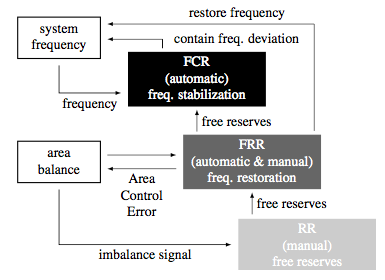
\includegraphics[width=7cm]{figures/reservesCategories.png}
	\caption{Reserve categories in ENTSO-E areas. \\ Graph taken from \citet{Stiphout2016}}
	\label{fig:reservesCategories}
\end{figure}

Since there is always a trade-off between the accuracy of technical constraints and computation time, which reserves should we take into account?
The expansion of renewable will put a particular emphasis on the need for FRR upwards reserve requirements. The requirements for downward reserves might be less stringent, as VRE should be able to participate in that market \citep{Stiphout2016, Hirth2015}.
As to RR, ENTSO-E sets no requirement for RR as it is not the main issue \citep{Stiphout2016}. 
Finally, FCR are determined by ENTSO-E for the area of Continental Europe, and this effort is then shared among the different countries. 
So in our model, we choose to insert upwards FRR requirements and FCR. We ignore downwards FRR reserve requirements and RR.

ENTSO-E provides guidelines as to the sizing of reserve requirements. The methode for sizing is well explained in \citet{Stiphout2016}:
\begin{quote}
	For each type of intermit-
	tent RES a probability density function (pdf) of the normalized forecast errors is introduced. This pdf is obtained by comparing the normalized day-ahead forecast with the normalized real-time output and describing the difference in a normal distribution. The 99\% quantile of this pdf is then the total FRR requirement. It dictates the required amount of MW of FRR per MW of installed RES capacity.
\end{quote}

The total FRR requirement is thus based on a probabilistic approach of the error forecasts. We use this approach here, base on RTE data for both wind\footnote{\url{https://clients.rteNAfrance.com/lang/fr/visiteurs/vie/previsions_eoliennes.jsp}} and PV\footnote{\url{https://clients,rteNAfrance,com/lang/fr/visiteurs/vie/prod/prevision_production,jsp?t=solaire}}.
Following the calculation protocol, we get the values of 0.027 for wind and 0.038 for solar.

The equation for reserves requirements is:

\begin{equation}
  \sum_{tec\_dispa} RES(tec\_dispa, y,w,h)   = \sum_{tec\_vre} epsilon(tec\_vre)*CAPA(tec\_vre,y) )
\end{equation}

\section{Power System Inflexibilities}

The model includes ramp-up and ramp-down constraints for nuclear and coal power plants, to represent the fact that generation cannot vary too quickly from one hour to the next.
We take the value of $0.08$ for coal and $0.05$ for nuclear - for both ramp-up and ramp-down, as in \citet{ADEME2015}.
These constraints are modelled as a maximum variation rate:
The ramp up constraint is:
\begin{multline}
  \forall tec\_dispa,y,w,h \quad GENE(tec\_dispa,y,w,h+1) \leq GENE(tec\_dispa,y,w,h) \\ + CAPA(tec\_dispa,y)*ramp\_rate(tec\_dispa)
\end{multline}
The ramp-down constraint is:
\begin{multline}
  \forall tec\_dispa,y,w,h \quad GENE(tec\_dispa,y,w,h+1) \geq GENE(tec\_dispa,y,w,h) \\ - CAPA(tec\_dispa,y)*ramp\_rate(tec\_dispa)
\end{multline}



\section{Model limitation}
This model was design to model the French power system from 2014 to 2050, optimizing investment and dispatch over many assumptions on nuclear costs. As such, it had to make several simplifying assumptions.

This model does not provide a detailed representation of infra-hourly events. In particular, ancillary services are not represented. 

We do not model power plants at the plant level, but we rather use representative technologies. Thus, one limitation is the absence of constraints related to unit commitment, such as start-up cost and delay, minimum load, and part-load efficiency. 
However, this default is in part compensated for nuclear. We use real data on age limit (or retirement), so the model retrofits plants whose capacity is in line with plant-level data. On the contrary, new nuclear will be installed continuously, while in reality it composed of discrete power plants with a significant size (1.3 GW for the EPR technology).
For renewable, the representative technology assumption is less of an issue as these technologies are modular, and very small in size. The continuous approach is here a good assumption for costs. However, this approach does not enable one to distinguish the different potentials within a country, both for solar and wind. 

%%%%%%%%%%%%%%%%

\clearpage

\section{Model Calibration}
\label{app:calibration}

The model is calibrated using capital cost, fixed O\&M and variable O\&M costs. 

Capital costs, O\&M costs and efficiency are taken from the World Energy Outlook: \url{http://www.worldenergyoutlook.org/weomodel/investmentcosts/}

Capital payments are annualized with a 8\% interest rate. This is in line with the range used in the literature. For example, \citet{Hirth2014} used an interest rate of 7\%.

The corresponding LCOE with usual load factor are given in the Figure \ref{fig:calibration_LCOE}.

\begin{figure}[!ht]
	\centering
	\includegraphics[width=12cm]{figures/calibration_LCOE.pdf}
	\caption{LCOE utilisés dans le modèle}
	\label{fig:calibration_LCOE}
\end{figure}

Then, we adapt the value for nuclear and renewable to France, for which more accurate data is available.
For new nuclear, we use the LCOE of the EPR project in Flamanville for 2015 (110 \emwh) and linearly reduce depending on the scenario for new nuclear costs. 

The LCOE reduces to 70\emwh in 2050 (low scenario), 90~\emwh~(medium scenario) or 110~\emwh~(high scenario).

For renewable, we start from the current feed-in tariffs, and decrease linearly to a long-term target depending on the renewable cost scenario. For the pessimistic renewable scenario, we use 60~\emwh~for wind and 50~\emwh~for solar. For the optimistic scenario, we reach 40~\emwh~for wind and 25~\emwh~for solar.
For wind, some EU action already yielded a price of 40~\emwh. spots.\footnote{\url{http://reneweconomy.com.au/eu-energy-auctions-yield-record-low-onshore-wind-prices-17917/}}
For solar, in Denmark, some auctions went below 13~\emwh.\footnote{\url{https://www.pv-magazine.com/2016/12/28/danish-solar-auction-delivers-european-low-cost-of-us-1-81-centskwh/}}
Thus, the costs I use have already been reached in some places , but I am trying to reproduce average costs, not the cost on the best spots. 

\begin{table}[!ht]
	\colorTable
	\centering
	\caption{Main model parameters}
	\begin{tabular}{llr}
		\toprule
		parameter&value&unit\\
		\midrule
		Rate of pure time preference &0&\%\\
		Financial interest rate&8&\%\\
		\bottomrule
	\end{tabular}
\end{table}

\begin{table}
	\centering
	\caption{Investment costs}
\label{tab:Investment _costs}
\small
	\begin{tabular}{llllllllllll}
		\toprule
		year & CCGT & coal & lake & nuc\_hist & nuc\_new & nuc\_retrofit & onshore & PV & river & step & TAC \\
		\midrule
		2015 & 1000 & 1700 & 2650 & 6600 & 6600 & 6600 & 1840 & 1320 & 3900 & 2650 & 500 \\
		2020 & 1000 & 1700 & 2650 & 6000 & 6000 & 6000 & 1780 & 1040 & 3900 & 2650 & 500 \\
		2030 & 1000 & 1700 & 2650 & 5100 & 5100 & 5100 & 1720 & 860 & 3900 & 2650 & 500 \\
		2040 & 1000 & 1700 & 2650 & 4500 & 4500 & 4500 & 1680 & 780 & 3900 & 2650 & 500 \\
		2050 & 1000 & 1700 & 2650 & 4500 & 4500 & 4500 & 1680 & 780 & 3900 & 2650 & 500 \\
		\bottomrule
	\end{tabular}
\end{table}


\begin{table}
	\centering
	\caption{Fixed O\&M costs}
	\label{tab:OM_costs}
	\small
	\begin{tabular}{llllllllllll}
		\toprule
		year & CCGT & coal & lake & nuc\_hist & nuc\_new & nuc\_retrofit & onshore & PV & river & step & TAC \\
		\midrule
		2015 & 25 & 45 & 80 & 170 & 170 & 170 & 45,67 & 13,5 & 60 & 20 & 15 \\
		2020 & 25 & 45 & 80 & 165 & 165 & 165 & 44 & 12 & 60 & 20 & 15 \\
		2030 & 25 & 45 & 80 & 165 & 165 & 165 & 44 & 12 & 60 & 20 & 15 \\
		2040 & 25 & 45 & 80 & 165 & 165 & 165 & 44 & 12 & 60 & 20 & 15 \\
		2050 & 25 & 45 & 80 & 165 & 165 & 165 & 44 & 12 & 60 & 20 & 15 \\
		\bottomrule
	\end{tabular}
\end{table}


\subsection{CO2 price}

For the \coo\ price, we consider three scenarios: low, medium and high price trajectories. In all three of them, we take the price up to 2017 equal to 10 euros/t\coo.
Then, for the high price trajectory, we take the value from \citet{Quinet2015}.
For the medium price trajectory, we choose a price increase which only half the one in the high scenario. For the low price trajectory, we choose a price increase which is only half the increase in the medium price trajectory.

\begin{table}
	\centering
	\caption{\coo\ price}
\label{tab:CO2_price}
	\begin{tabular}{llll}
		\toprule
		Year & High & Medium & Low \\
		\midrule
		2015 & 10 & 10 & 10 \\
		2020 & 56 & 33 & 21,5 \\
		2030 & 100 & 55 & 32,5 \\
		2040 & 150 & 80 & 45 \\
		2050 & 200 & 105 & 57,5 \\
		\bottomrule
	\end{tabular}
\end{table}



\subsection{Demand}

The demand in 2030 and 2050 was taken from \citet{Grandjean2014}. However, due to the very high increase in the DEC scenario, we halve its increase by a factor two. The evolution of demand for each scenario is shown in figure \ref{fig:demand_evolution}.

\begin{figure}[!ht]
	\centering
	\includegraphics[width=6cm]{figures/demand_evolution.pdf}
	\caption{Demand evolution in our four demand scenarios}
	\label{fig:demand_evolution}
\end{figure}

\subsection{Exogenous capacities}

For the capacities of historical nuclear, we take the date of the fourth ten-year inspection by the Nuclear Safety Authority, which provides the legal authorization to run. These values depart slightly from 40 years for each plants, because of slight lags at each inspection. 
The cumulative available capacity before retrofit is given in figure , which illustrate the challenge of the nuclear cliff.

\begin{figure}[!ht]
	\centering
	\includegraphics[width=6cm]{figures/nuclear_cliff.pdf}
	\caption{Available nuclear capacities without retrofitting}
	\label{fig:nuclear_cliff}
\end{figure}

Additionally, we suppose the EPR will start in 2020, due to the most recent announcements which mentions full charge will be reach in November 2019.

As to hydro-related capacities, we assume constant capacities for run-of-river and lakes. Pumped-hydro potential is expected to grow by 3.2GW by 2050, starting from 5 GW in 2014, with a discharge time of 20 hours, as in \citet{ADEME2013}.
$$CAPA(tec\_ex,y) = capa\_exo_(y,tec\_ex) $$

\subsection{Fuel prices}

\begin{table}[!ht]
	\centering
	\caption{Fuel prices}
	\label{tab:Fuel_prices}
	\begin{tabular}{llll}
		\toprule
		euro/MWh & Coal & Gas & Uranium \\
		\midrule
		2014 & 10.3 & 25.3 & 7.30 \\
		\bottomrule
	\end{tabular}
\end{table}

\subsection{Fuel efficiencies}

\begin{table}[!h]
	\centering
	\caption{Efficiencies}
	\label{tab:Efficiencies}
	\begin{tabular}{lll}
		\toprule
		Coal & CCGT & TAC \\
		\midrule
		0,43 & 0,61 & 0,410 \\
		\bottomrule
	\end{tabular}
\end{table}

\subsection{Capex annuities}

We assume that the overnight cost is paid with constant annuities.
Capital annuities are equal to the overnight cost multiplied by the capital recovery factor (CRF). The formula to compute constant annuities is:
$$\text{Annuities} = \text{Overnight cost} \cdot \frac{i}{1 - (1+i)^{-N}} $$
where $i$ is the interest rate and $N$ is the number of years, i.e. the lifetime of the plant.

The LCOE can then be computed with the formula:
$$\text{LCOE} = \frac{ \text{Annuity} + \text{fixed O\&M} } { \text{Number of hours of generation at full power}} +  \text{variable costs}$$

\subsection{Deployment speed}

The maximum deployment speed for each technology is given in table \ref{tab:deploy_speed}. In particular, we set it to 4~GW/year for wind and 6~GW/year for solar, which are roughly equal to the average maximum deployment speed in Germany. For nuclear, we set it to 2.3~GW/year, which is equal to 2 new EPR reactor per year.

\begin{table}[!h]
	\centering
	\caption{Maximum deployment speed}
	\label{tab:deploy_speed}
	\begin{tabular}{lc}
		\toprule
		Technology & Capacity \\
		 & (GW/year) \\
		\midrule
		onshore & 4 \\
		PV & 6 \\
		coal & 4 \\
		CCGT & 4 \\
		TAC & 4 \\
		nuc\_retrofit & 4 \\
		nuc\_new & 2.3 \\
		\bottomrule
	\end{tabular}
\end{table}


\clearpage

\section*{Bibliography}
\bibliography{Collection}


\end{document}
